% !TeX spellcheck = en_US
\documentclass[letterpaper,12pt,twoside]{report}
\usepackage{fancyhdr}
\usepackage{fullpage}
\usepackage{tikz}
\usepackage{amsmath}
\usepackage{xcolor}

\begin{document}
	\pagestyle{fancy}
	\fancyhf{}
	\fancyhead[L]{Day 9}
	\fancyhead[R]{\textit{The Calendar Project}}
	\fancyfoot[L]{Citations Involved: none}
	
	% Problem
	\paragraph{Problem}
	\begin{quote}
		\textsf{Three vertices of a regular hexagon are selected at random, without replacement. What is the probability that the selected vertices form an isosceles or an equilateral triangle?}
	\end{quote}
	
	% Graphics
	\begin{center}
		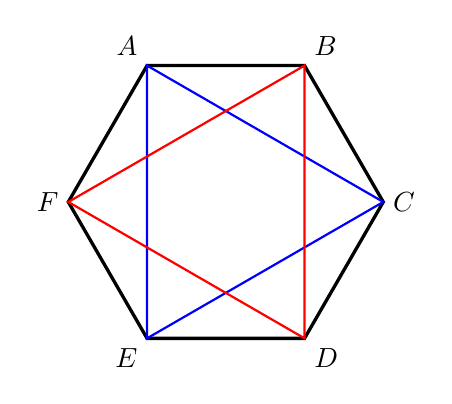
\begin{tikzpicture}
		\draw[very thick] (2,0) -- (1,-1.732) -- (-1,-1.732) -- (-2,0) -- (-1,1.732) -- (1,1.732) -- cycle;
		
		\draw[thick][blue] (-1,1.732) -- (2,0) -- (-1,-1.732) -- cycle;
		\draw[thick][red] (1,1.732) -- (1,-1.732) -- (-2,0) -- cycle;
		
		\node[above left] at (-1,1.732) {$A$};
		\node[above right] at (1,1.732) {$B$};
		\node[right] at (2,0) {$C$};
		\node[below right] at (1,-1.732) {$D$};
		\node[below left] at (-1,-1.732) {$E$};
		\node[left] at (-2,0) {$F$};
		
		\end{tikzpicture}
	\end{center}
	
	% Reasoning
	\paragraph{Reasoning}
	\begin{quotation}
		
		\textbf{There are two equilateral triangles that can be constructed from three of the hexagon's vertices}---they are denoted in \textcolor{red}{red} and \textcolor{blue}{blue} above (this can be proven with the hexagon's sides using SAS triangle congruency). Since the sides of a regular polygon are congruent (1), triangles constructed from two consecutive sides of the regular hexagon are isosceles. Since each vertex corresponds to a unique pair of consecutive sides, and since there are six pairs of consecutive sides in the hexagon, \textbf{there are six isosceles triangles that can be constructed from three of the hexagon's vertices}.
		
		Since a hexagon has 6 vertices by definition, there are ${}_6 C_3=20$ ways to choose three vertices from a hexagon, disregarding order.
		
		$P(A \textrm{\space or } B)=P(A)+P(B)$ (2). Let $A$ be the condition that an isosceles triangle can be formed, and let $B$ be the condition that an equilateral triangle can be formed. Applying $\frac{\text{favorable}}{\text{all possible}}$, it is determined that $P(A)=\frac{6}{20}=\frac{3}{10}$ and $P(B)=\frac{2}{20}=\frac{1}{10}$. Thus the solution to this problem is $P(A)+P(B)=\frac{3}{10}+\frac{1}{10}=\frac{4}{10}=\boxed{\frac{2}{5}}$.
		
	\end{quotation}
	
	\paragraph{External References}
	
	\begin{enumerate}
		\item Textbook, Ch. 6, Pg. 382: Definition of a Regular Polygon
		\item Textbook, Ch. 13, Pg. 907: Mutually Exclusive Events
	\end{enumerate}
	
\end{document}